\documentclass[12pt,twoside]{report}
\usepackage[a4paper,left=20mm,right=20mm,top=25mm,bottom=25mm,headheight=15pt]{geometry}
\usepackage[utf8]{inputenc}
\usepackage{graphicx}
\graphicspath{ {images/} }
\usepackage{lipsum}

% Font
\usepackage{titlesec}
\usepackage{fontspec}
\defaultfontfeatures{Ligatures=TeX} 
\setsansfont{Lato}[
	Path = fonts/Lato/,
	Extension = .otf,
	UprightFont = *-Regular,
	BoldFont = *-Bold,
	ItalicFont = *-Italic,
	BoldItalicFont = *-BoldItalic,
]
\setmonofont{SourceCodePro}[
	Path = fonts/SourceCodePro/,
	Extension = .otf,
	UprightFont = *-Regular,
	BoldFont = *-Bold,
	ItalicFont = *-Italic,
	BoldItalicFont = *-BoldItalic,
]
\setmainfont{Newsreader}[
	Path = fonts/Newsreader/,
	Extension = .otf,
	UprightFont = *-Regular,
	BoldFont = *-Bold,
	ItalicFont = *-Italic,
	BoldItalicFont = *-BoldItalic,
]

\titleformat{\chapter} % type of title to format
    [display] % shape
    {\sffamily\Huge\bfseries\raggedleft} % how to format it
    {\thechapter} % label
    {0pt} % seperator between label and the chapter name below it.
    {\titlerule\vspace{2pt}\titlerule[1pt]\vspace{5pt}}

\titleformat{\section}
    {\sffamily\Large\bfseries}
    {\thesection}
    {1em}
    {}
\titleformat{\subsection}
    {\sffamily\large\bfseries}
    {\thesubsection}
    {1em}
    {}
\titleformat{\subsubsection}
    {\sffamily\normalsize\bfseries}
    {\thesubsubsection}
    {1em}
    {}

% code
\usepackage{minted}
\setminted{fontsize=\small}
\usemintedstyle{solarized-light}

% Set headers
\usepackage{fancyhdr}
\fancypagestyle{custom}{
	\fancyhf{}
	\fancyhead[RE]{\sffamily{\thepage}}
	\fancyhead[LO]{\sffamily{\thepage}}
	\fancyhead[LE]{\sffamily{\rightmark}}
	\fancyhead[RO]{\sffamily{\leftmark}}
	\renewcommand{\headrulewidth}{0pt}
	\renewcommand{\footrulewidth}{0pt}
}
\pagestyle{custom}
% Override Chapter pages where the report document class sets \thispagestyle{plain}
\fancypagestyle{plain}{
    \fancyhf{}
    \fancyfoot[C]{\sffamily{\thepage}}
}

\pagenumbering{arabic}

\begin{document}
    \begin{titlepage}
    \begin{center}
        \vspace*{1cm}
        \textbf{Report Title}
        \vspace{0.5cm}

        Report subtitle
        \vspace{1.5cm}

        \textbf{Kristian Nymann Jakobsen} 
        \vspace{0.5cm}

        \texttt{kjako19@student.sdu.dk}
        \vfill

        Course
        \vspace{0.8cm}

        \includegraphics[width=0.4\textwidth]{university}
        \vspace{0.5cm}

        The Faculty of Engineering \\
        University of Southern Denmark\\
        \date{\today}
    \end{center}
\end{titlepage}

    \newpage
    
    \setcounter{page}{0}
\setcounter{tocdepth}{2} % anything below subsection will not be added
\tableofcontents
\thispagestyle{empty}

    \newpage
    
    \chapter{Part One}
    \section{Code}
\subsection{Python}
\begin{minted}{python}
import sys
import fontforge

def convert_to_otf(path: str):
    font = fontforge.open(path)
    new_file_name = path.replace(".ttf", ".otf")
    font.generate(new_file_name)

if __name__ == "__main__":
    for p in sys.argv[1:]:
        convert_to_otf(p)
\end{minted}

\subsection{AWK}
\subsubsection{Password-File Checking}
The password file on a Unix system contains the name of and other information
about authorized users. Each line of the password file has 7 fields, seperated
by colons:
\small\begin{verbatim}
    root:qyxRi2uhuVjrg:0:2::/:
    bwk:1L./v6iblzzNE:9:1:Brian Kerninghan:/usr/bwk:
    ava:otxs1oTVoyvMQ:15:1:Al Aho:/usr/ava:
    uucp:xutIBs2hKtcls:48:1:uucp daemon:/usr/lib/uucp:uucico
    pjw:xNqy//GDc8FFg:170:2:Peter Winberger:/usr/pjw:
    mark:j0z1fuQmqIvdE:374:1:Mark Kernighan:/usr/bwk/mark:
    ...
\end{verbatim}
\normalsize
The first field is the user's login name, which should be alphanumeric. The
second is an encrypted version of the password; if this field is empty, anyone
can log in pretending to be that user, while if there is a password, only
people who know the password can log in. The third and fourth fields are
supposed to be numeric. The sixth field should begin with /. The following
program prints all lines that fail to satisfy these criteria, along with the
number of the erroneous line and an approritate diagnostic message. Running
this program every night is a small part of keeping a system healthy and safe
from intruders.

\begin{minted}{awk}
    # passwd - check password file

    BEGIN {
        FS = ":" }
    NF != 7 {
        printf("line %d, does not have 7 fields: %s\n", NR, $0) }
    $1 ~ /[^A-Za-z0-9]/ {
        printf("line %d, nonalpanumeric user id: %s\n", NR, $0) }
    $2 == "" {
        printf("line %d, no password: %s\n", NR, $0) }
    $3 ~ /[^0-9]/ {
        printf("line %d, nonumeric user id: %s\n", NR, $0) }
    $4 ~ /[^0-9]/ {
        printf("line %d, nonnumeric group id: %s\n", NR, $0) }
    $6 !~ /^\// {
        printf("line %d, invalid login directory: %s\n", NR, $0) }
\end{minted}


\section{Slanted}
\textsl{\lipsum[1]}

\section{Italic}
\textit{\lipsum[2]}

\section{Bold}
\textbf{\lipsum[4]}


    \chapter{Part Two}
    \section{Client Server}
For this part of the assignment, I chose to use UTF based sockets. The reason
for this, is that they are simple to use and fit the requirement well (we are
only interested in the value and not timestamp, etc.).

\begin{figure}
\caption{Sensor Client}
\centering
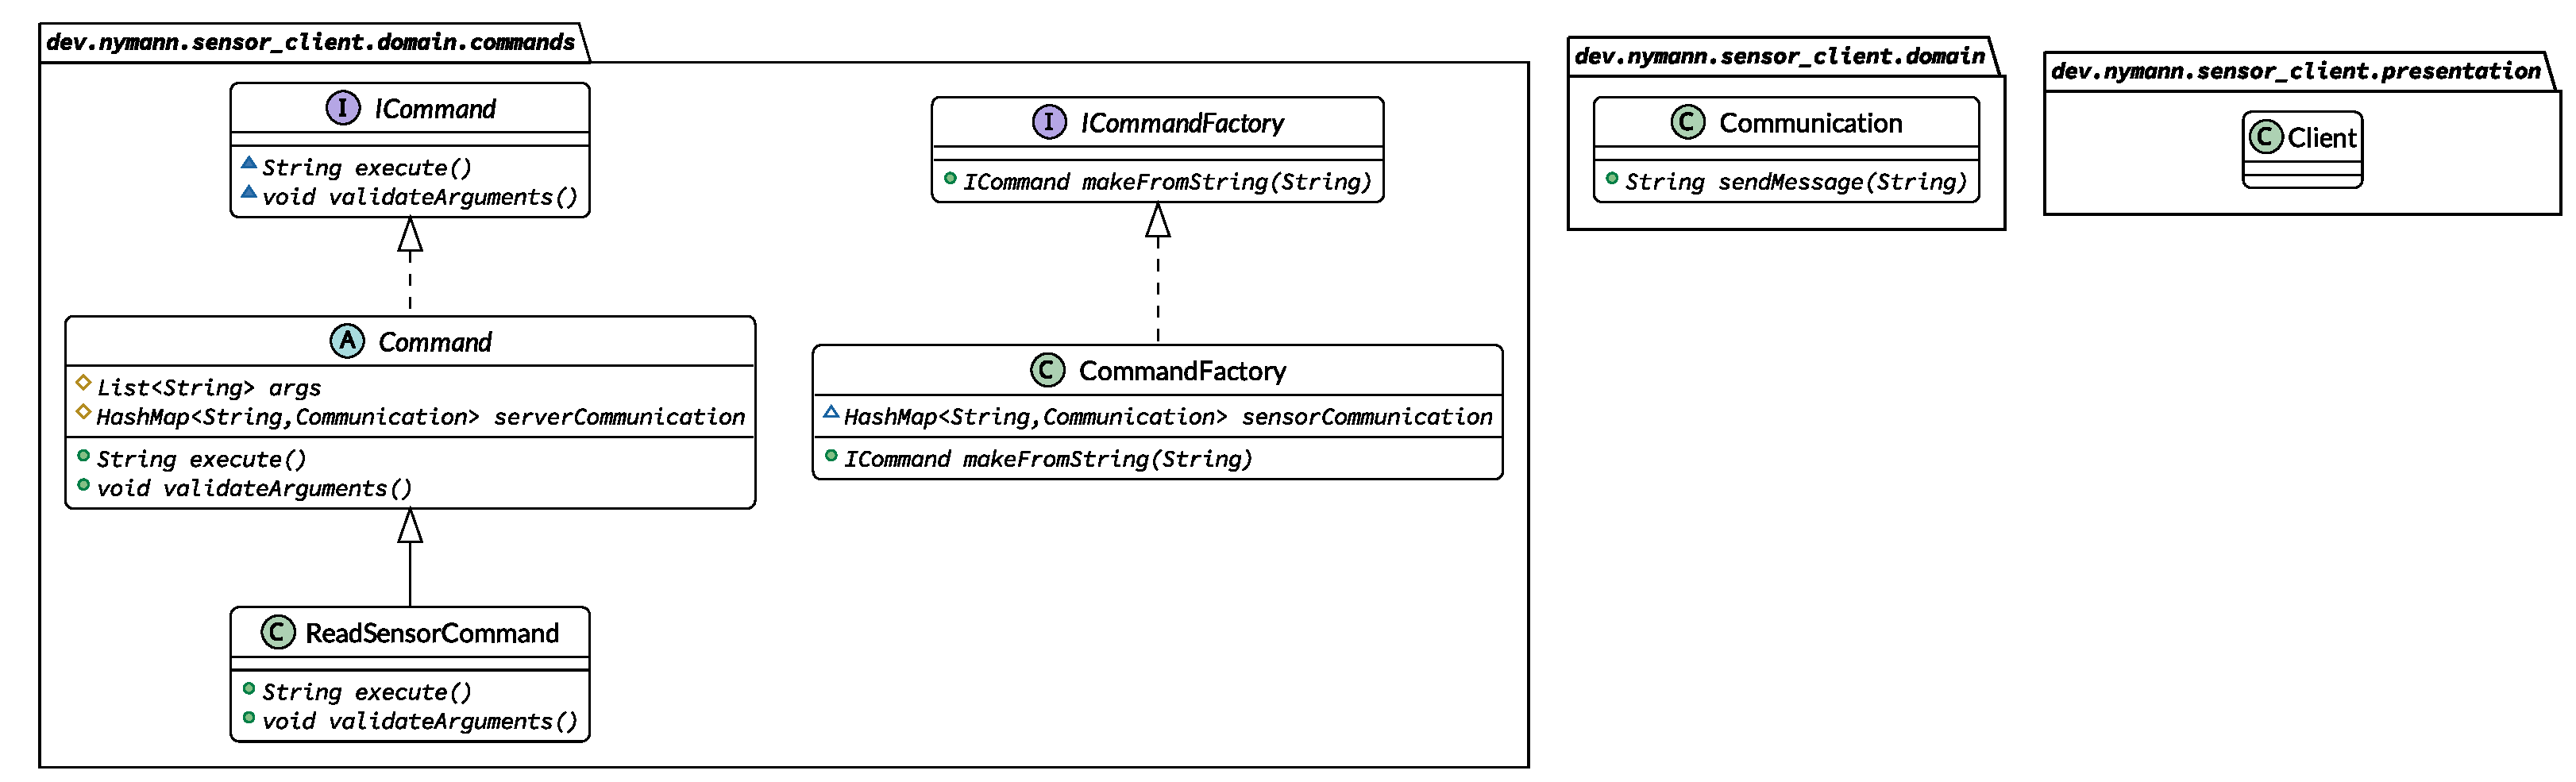
\includegraphics[scale=0.3]{part_two/sensor-client}
\end{figure}

\begin{figure}
\caption{Sensor Server}
\centering
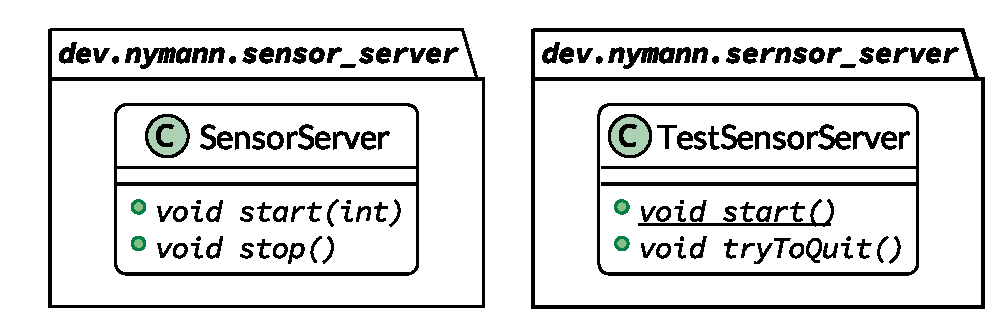
\includegraphics[scale=0.8]{part_two/sensor-server}
\end{figure}

\begin{figure}
\caption{Sensor}
\centering
\includegraphics[scale=0.8]{part_two/sensor}
\end{figure}

\begin{figure}
\caption{CO2 Sensor}
\centering
\includegraphics[scale=0.8]{part_two/co2-sensor}
\end{figure}

\begin{figure}
\caption{CO2 Sensor}
\centering
\includegraphics[scale=0.8]{part_two/temperature-sensor}
\end{figure}


    \chapter{Part Three}
    \section{Hazelcast Map}
The source code for this part can be found inside the
\small\texttt{src/portfolio\_assignment\_part\_three}
\normalsize directory.

\begin{figure}
\caption{Sensor Client}
\centering
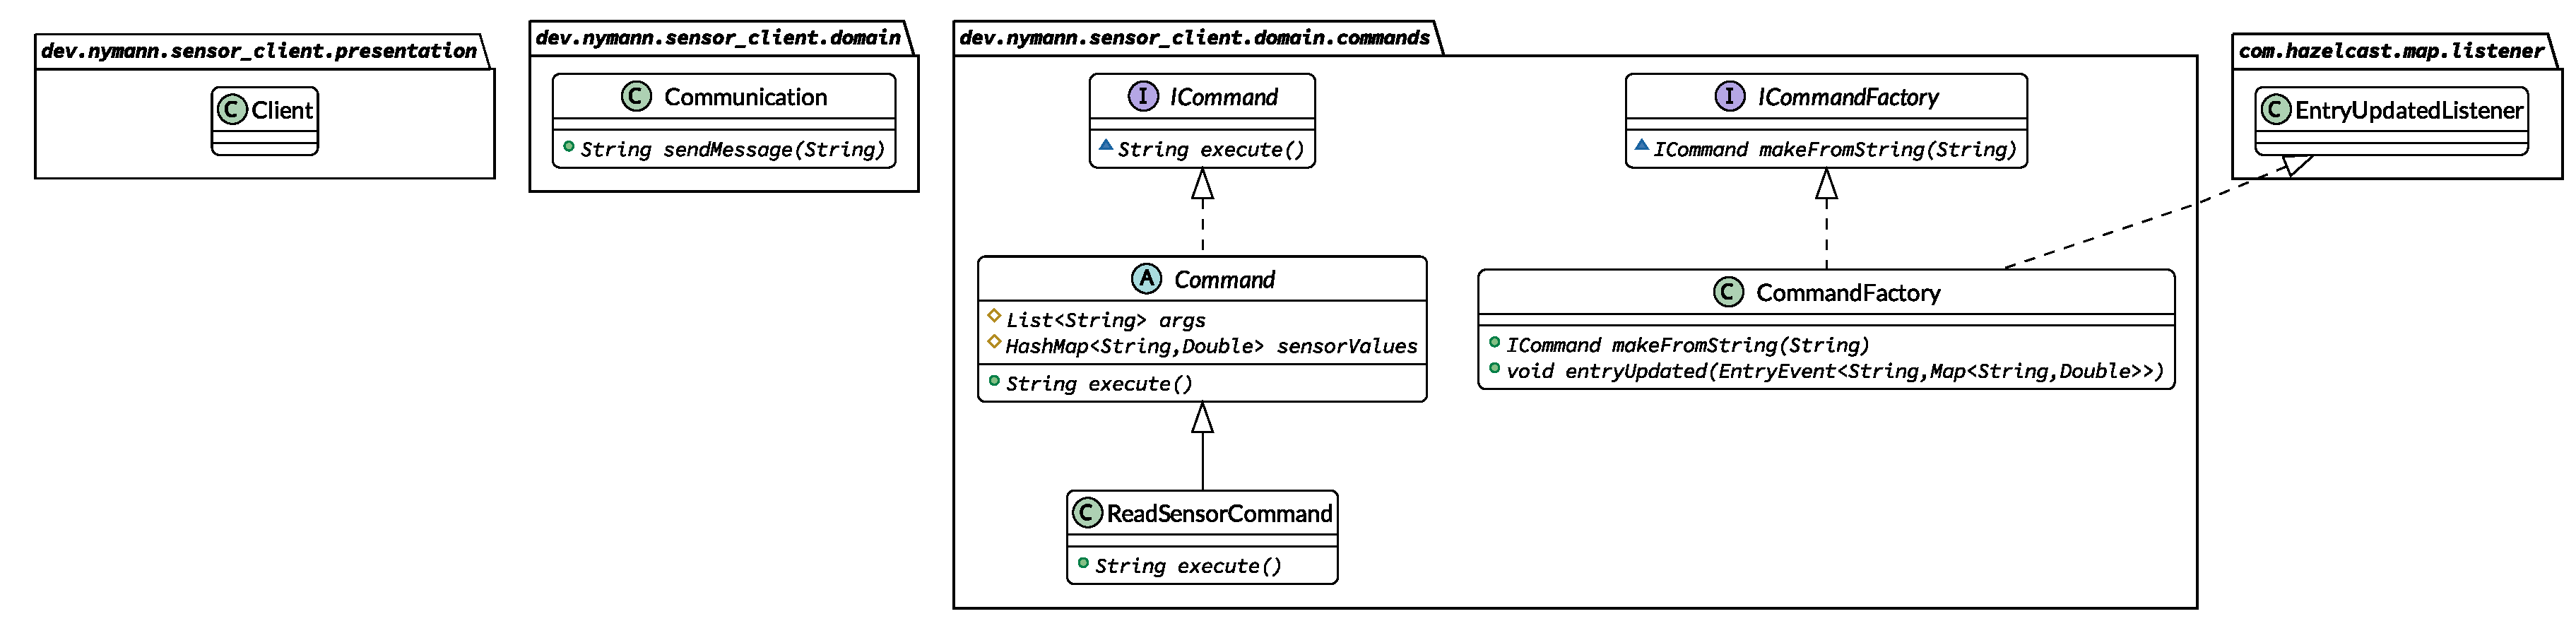
\includegraphics[scale=0.3]{part_three/sensor-client}
\end{figure}

\begin{figure}
\caption{Sensor Server}
\centering
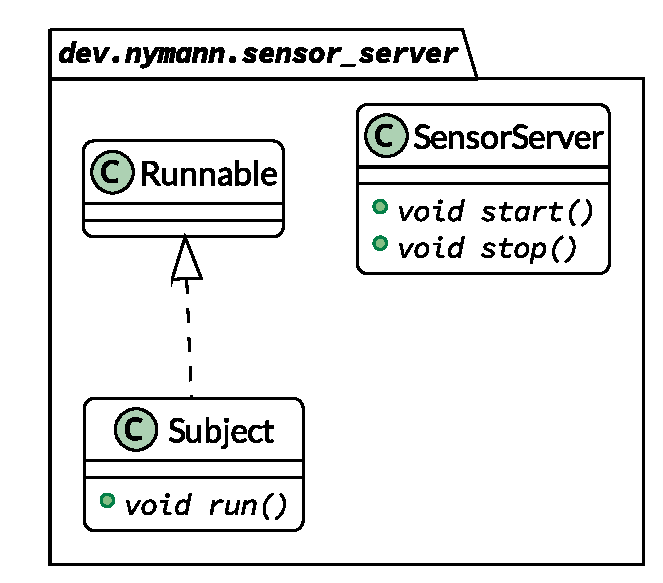
\includegraphics[scale=0.8]{part_three/sensor-server}
\end{figure}

\begin{figure}
\caption{Sensor}
\centering
\includegraphics[scale=0.8]{part_three/sensor}
\end{figure}

\begin{figure}
\caption{CO2 Sensor}
\centering
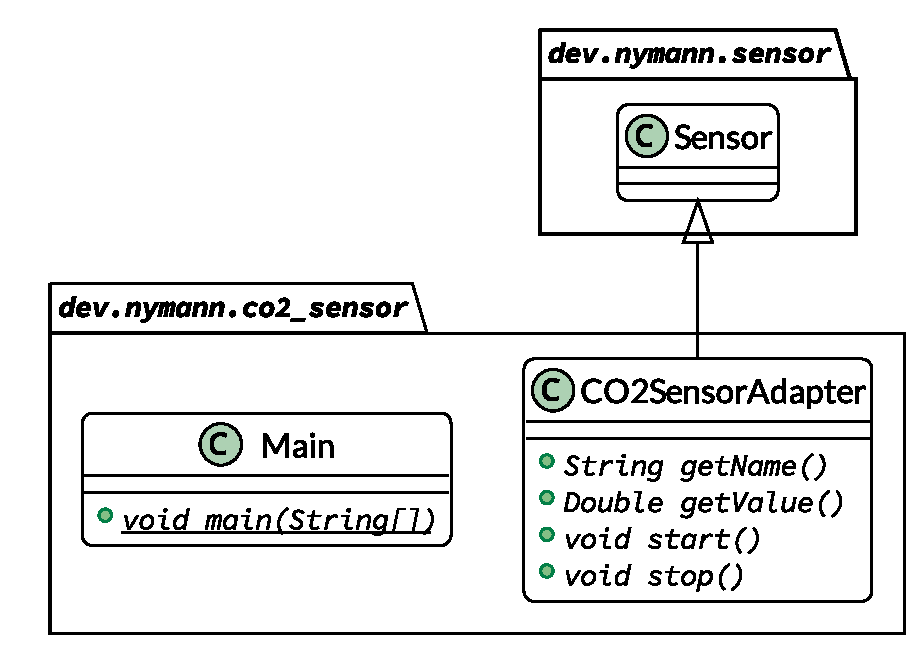
\includegraphics[scale=0.8]{part_three/co2-sensor}
\end{figure}

\begin{figure}
\caption{CO2 Sensor}
\centering
\includegraphics[scale=0.8]{part_three/temperature-sensor}
\end{figure}


    \chapter{Part Four}
    \section{Hazelcast Topic}
The source code for this part can be found inside the
\small\texttt{src/portfolio\_assignment\_part\_four}
\normalsize directory.

\begin{figure}
\caption{Sensor Client}
\centering
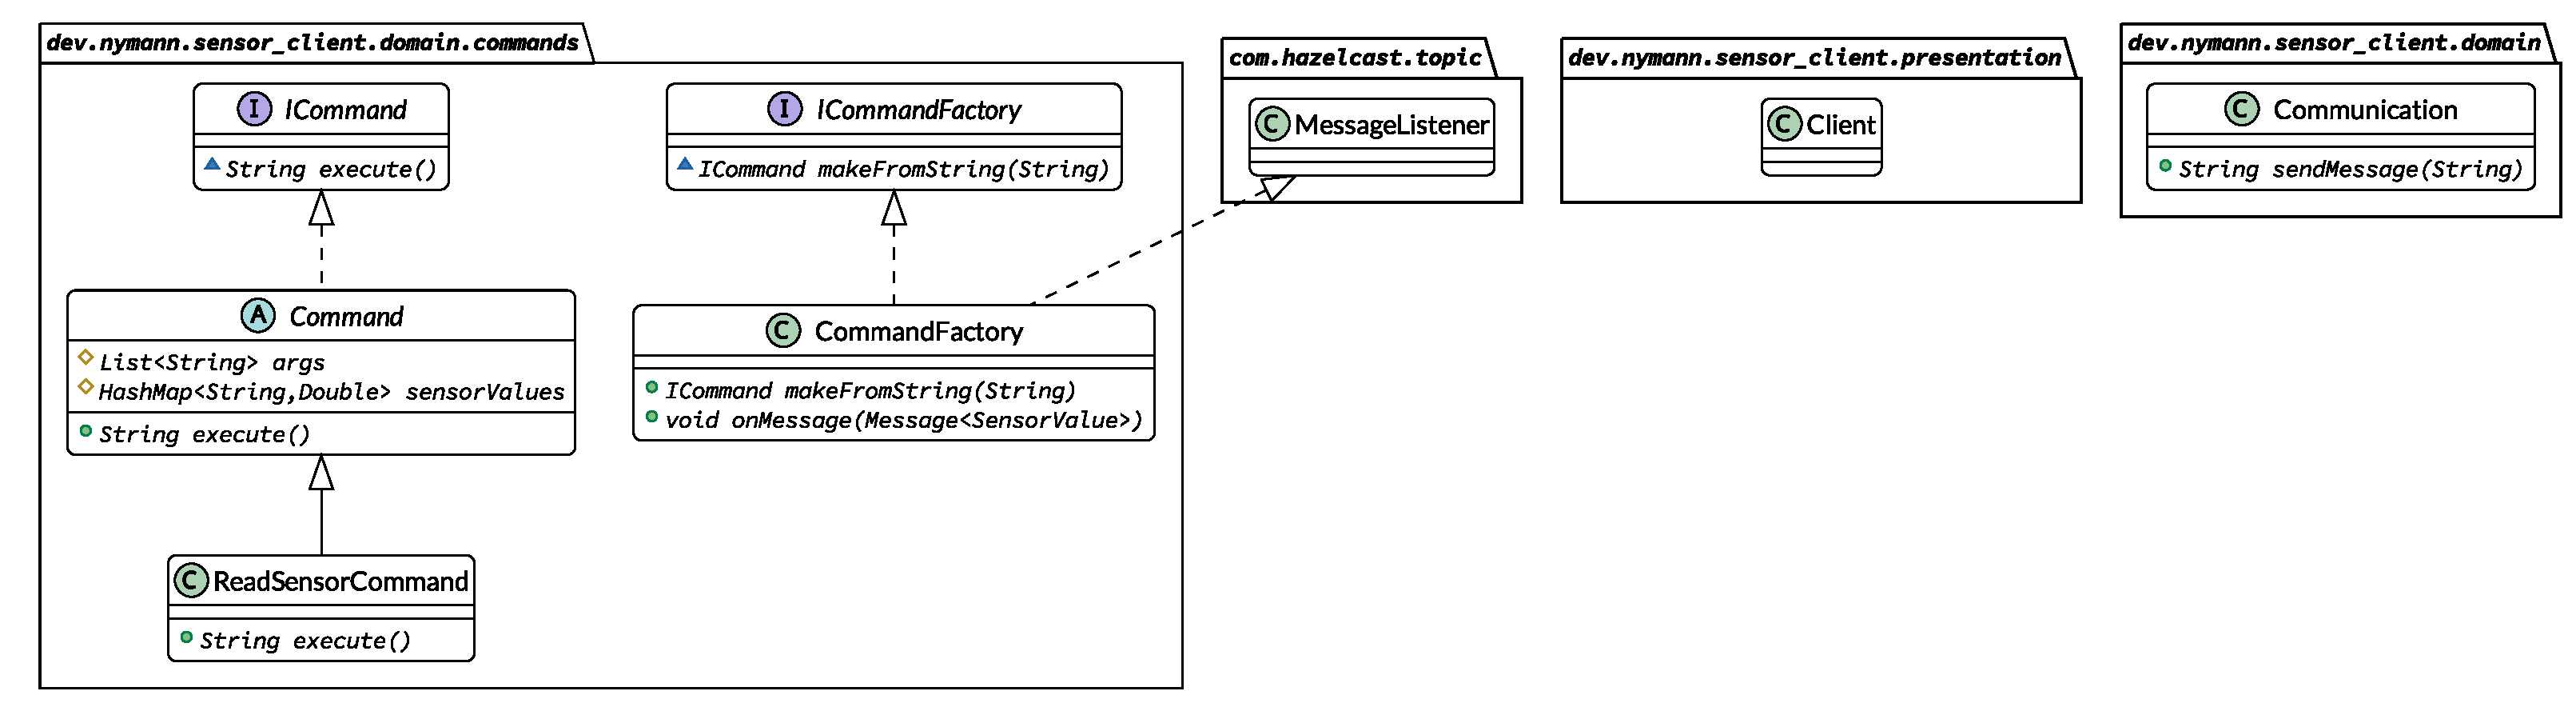
\includegraphics[scale=0.3]{part_four/sensor-client}
\end{figure}

\begin{figure}
\caption{Sensor Server}
\centering
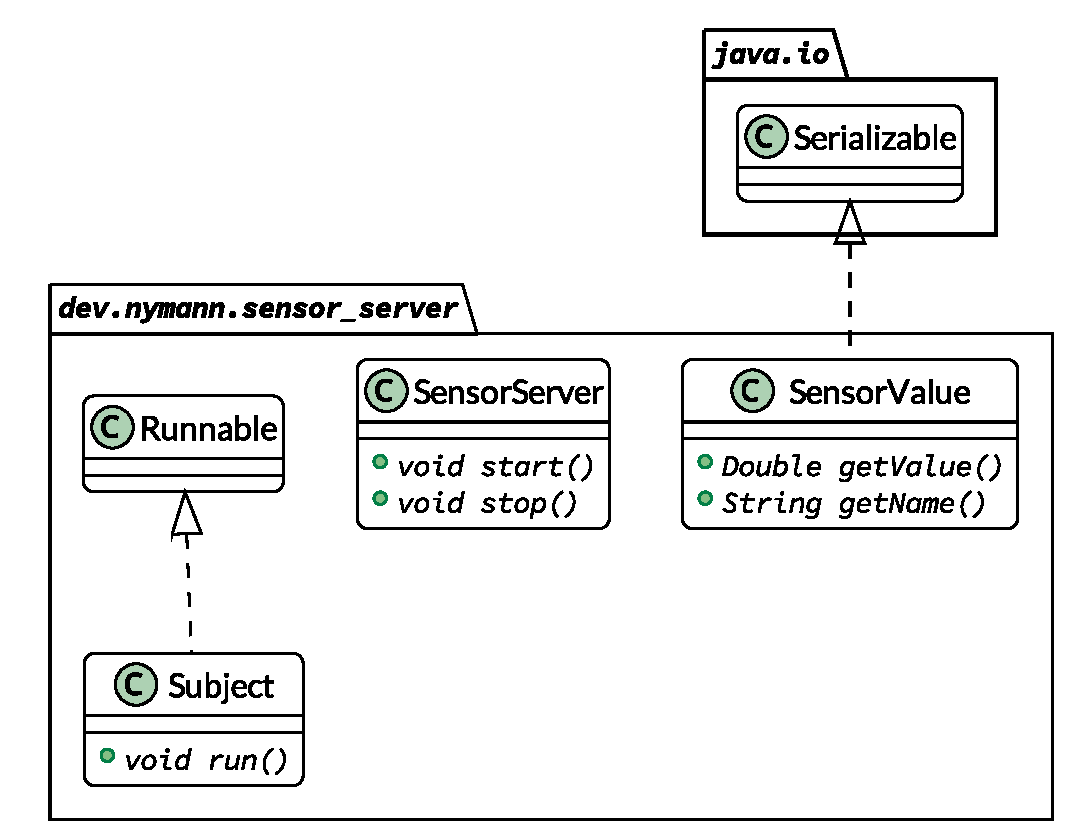
\includegraphics[scale=0.8]{part_four/sensor-server}
\end{figure}

\caption{Sensor}
\begin{figure}
\centering
\includegraphics[scale=0.8]{part_four/sensor}
\end{figure}

\begin{figure}
\caption{CO2 Sensor}
\centering
\includegraphics[scale=0.8]{part_four/co2-sensor}
\end{figure}

\begin{figure}
\caption{CO2 Sensor}
\centering
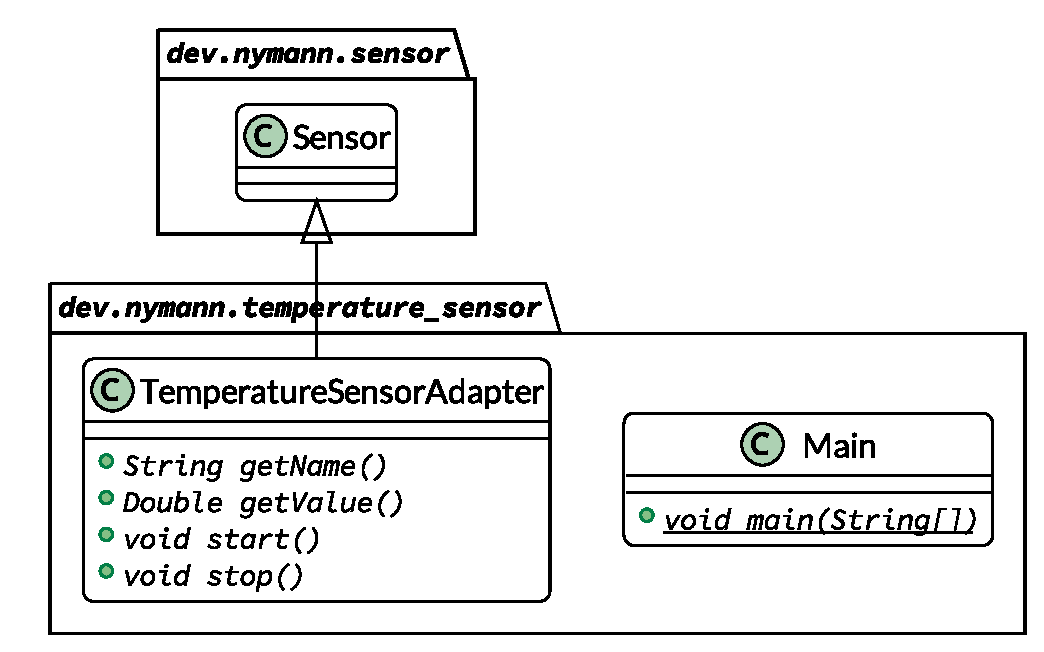
\includegraphics[scale=0.8]{part_four/temperature-sensor}
\end{figure}

\end{document}
